% ===========================================================================
\section{An Energy-Based SFPRM}
\label{sec:energy}

\Cref{sec:differences} identified the energy as the main structural difference between the two
models: AKOrN's drive is a gradient field when $J$ is symmetric, whereas SFPRM's $F_\theta$ never is.
We now close this gap from the SFPRM side. The recurrent map is replaced by a Riemannian gradient
step on an explicit energy $E(w;x)$, so that every iteration is an AKOrN step whose drive is
$-\nabla E$. The injection is already a gradient (\cref{prop:injection-gradient}); for attention
and the MLP we take the two energies of the Energy Transformer \citep{hoover2023et} to the sphere,
with modifications that reasoning tasks turn out to require (\cref{sec:energy-design}).

\subsection{Energy, Update and Gradient}
\label{sec:energy-def}

\begin{definition}[Energy SFPRM]
\label{def:esfprm}
The state is $w=(z,u)\in(\Sph^{d-1})^{2T}$ with visible tokens $z$ and hidden tokens $u$, one per
visible token; the \emph{flat} variant identifies $u\equiv z$. With heads $k=1,\dots,H$, signed head
weights $\sigma_k\in\R$, logit scales $\beta_k>0$, memories $\xi_1,\dots,\xi_K\in\R^d$ (rows of
$\Xi$) and $\kappa_0,\kappa_C,\kappa_M,\beta_M>0$,
\begin{equation}
\begin{aligned}
  E(w;x) &= \kappa_0\,\Phi_x(z) + E_A(u,z) + E_C(u,z) + E_M(u),\\
  E_A &= -\textstyle\sum_{k=1}^H\frac{\sigma_k}{\beta_k}\sum_{t}\log\sum_{s\neq t}e^{\ell^k_{ts}},\\
  E_C &= -\kappa_C\textstyle\sum_t\ip{u_t}{Cz_t},\\
  E_M &= -\frac{\kappa_M}{\beta_M}\textstyle\sum_t\log\sum_{\mu=1}^Ke^{\beta_M\ip{\xi_\mu}{u_t}},
\end{aligned}
\label{eq:energy}
\end{equation}
where $\ell^k_{ts}:=\beta_k\ip{W_Q^ku_t}{W_K^kz_s}$ are the attention logits and
$\Phi_x(z)=\tfrac12\sum_t\angle(z_t,x_t)^2$ is the injection potential of
\cref{prop:injection-gradient}. The recurrent map is the unit gradient step
$F_E(w;x):=\Exp_w\big(-\grad E(w;x)\big)$, with $\grad$ the Riemannian gradient on
$(\Sph^{d-1})^{2T}$, and the iteration is SFPRM's damped loop \eqref{eq:sfprm-damp} with $F_E$ in
place of $F_\theta$:
\begin{equation}
\begin{aligned}
  w_{i+1}&=\Slerp_{\eta_i}\big(w_i,F_E(w_i;x)\big)\\&=\Exp_{w_i}\big(-\eta_i\grad E(w_i;x)\big),
\end{aligned}
  \label{eq:esfprm-step}
\end{equation}
the equality by \cref{lem:slerp} whenever $\norm{\grad_{w_t}E}<\pi$. The prediction is read from
$z$. SFPRM's chordal halting residual of $F_E$ is $1-\cos\norm{\grad_{w_t}E}$, so the halting test
is $\max_t\norm{\grad_{w_t}E}<\tau_g$: the iteration halts at $\tau_g$-stationary points of $E$.
\end{definition}

\begin{proposition}[The gradient is injection, symmetric coupling and memory]
\label{prop:energy-gradient}
Let $a^k_{ts}=\operatorname{softmax}_{s\neq t}\big(\beta_k\ip{W_Q^ku_t}{W_K^kz_s}\big)$ and
$M_k:=(W_Q^k)^\top W_K^k$. Token-wise,
\begin{align}
  -\grad_{z_t}E &= \kappa_0\Log_{z_t}x_t+\kappa_C\Proj_{z_t}C^\top u_t\nonumber\\
  &\quad+\Proj_{z_t}\textstyle\sum_k\sigma_k\sum_{s\neq t}a^k_{st}M_k^\top u_s,\label{eq:grad-z}\\
  -\grad_{u_t}E &= \Proj_{u_t}\Big[\textstyle\sum_k\sigma_k\sum_{s\neq t}a^k_{ts}M_kz_s\nonumber\\
  &\quad+\kappa_CCz_t+\kappa_M\Xi^\top\!\operatorname{softmax}(\beta_M\Xi u_t)\Big].\label{eq:grad-u}
\end{align}
In the flat variant the two attention sums add, and the drive is an AKOrN coupling $\sum_sJ_{ts}(z)z_s$
with $J_{ts}=\sum_k\sigma_k\big(a^k_{ts}M_k+a^k_{st}M_k^\top\big)$, which satisfies AKOrN's
symmetry condition $J_{ts}=J_{st}^\top$ at every state.
\end{proposition}

Every term has a counterpart in \cref{thm:trotter}: $\kappa_0\Log_zx$ is the stimulus $c$, the
attention sums are the coupling $Jz$, and the memory is the self-drive $m$. The energy model is
therefore the collapsed single-step form of SFPRM in which the coupling is a gradient field and the
MLP is a Hopfield memory: the query-path term $\sum_sa_{ts}M_kz_s$ is standard attention with value
matrix $M_k$ (rank at most $d_h$), the key-path term $\sum_sa_{st}M_k^\top u_s$ is the
contribution that makes the field conservative \citep{hoover2023et}, the matrix $C$ plays the role
of the output projection, and $\Xi^\top\operatorname{softmax}(\beta_M\Xi u)$ is the tied-weight MLP
$W_2\,r(W_1u)$ with $W_2=W_1^\top$ and $r=\operatorname{softmax}$, the retrieval rule of modern
Hopfield networks \citep{krotov2016dam,ramsauer2021hopfield}; $r=\operatorname{relu}$ with
$G(a)=\tfrac12\operatorname{relu}(a)^2$ in place of the log-sum-exp gives the classical memory.
In the terms of \cref{tab:differences}, the energy row now reads ``yes'' for both models.

\subsection{Three Design Choices}
\label{sec:energy-design}

The Energy Transformer was designed for image completion and graph tasks. Three modifications,
each forced by a failure we observed in the pilot of \cref{sec:energy-pilot}, make
\eqref{eq:energy} suitable for reasoning while keeping it an energy.
\emph{Signed heads.} With $\sigma_k>0$ the log-sum-exp is minimized by aligning queries with keys:
attention is attractive. A head with $\sigma_k<0$ is repulsive, and its drive pushes a token away
from the tokens it attends to most. Constraints of the form ``cells in the same unit hold different
digits'' are repulsive couplings, the negative couplings of the Kuramoto model
\citep{kuramoto1984}, and cannot be expressed with attractive heads alone.
\emph{Hidden tokens.} In the flat variant the message $M_kz_s$ delivered to a token is tied to the
score $\ip{W_Q^kz_t}{W_K^kz_s}$ that selects it, since both use $M_k$; a model cannot match on
position and message on content. Hidden tokens receive the query-path message, the visible token
receives $C^\top u_t$ through the free bilinear coupling $E_C$, and matching and messaging decouple.
The energy becomes a two-layer associative memory \citep{krotov2021hierarchical}; the state doubles,
the theory below is unchanged.
\emph{Sharpness versus message size.} In \eqref{eq:energy} the softmax sharpness is
$\beta_k\norm{W_Q^ku_t}\norm{W_K^kz_s}$ while the message size is $|\sigma_k|\norm{M_kz_s}$, so a
small $W$ with a large $\beta_k$ gives sharp attention and unit-scale messages at the same time, the
separation that QK-normalization and the logit scale achieve in nGPT. Sizing $W$ for unit logits
instead makes $\norm{M_k}$ large, the Hessian of $E_A$ grows with $\beta_k\norm{M_k}^2$, and the
iteration leaves the stability window of \cref{prop:real-spectrum}.

\subsection{What the Energy Buys}
\label{sec:energy-theory}

\begin{theorem}[Energy descent, global convergence and a halting bound]
\label{thm:lyapunov}
Let $L>0$ be such that $E(\Exp_w(v))\le E(w)+\ip{\grad E(w)}{v}+\tfrac L2\norm v^2$ for all $w$ and
tangent $v$. Such an $L$ exists; $L=\sup_w\lambda_{\max}(\operatorname{Hess}E(w))$ suffices, and the
injection contributes at most $\kappa_0$ to it because the Hessian of $\tfrac12\angle(\cdot,x)^2$ has
eigenvalues $1$ and $\theta\cot\theta\le1$. Fix $\eta\in(0,2/L)$ and let $c_\eta:=\eta(1-\eta L/2)>0$.
Then along every trajectory on which no token is antipodal to its input (an exceptional set of
measure zero, empty for the chordal injection $\sum_t(1-\ip{z_t}{x_t})$):
\begin{enumerate}
  \item[(i)] $E(w_{i+1})\le E(w_i)-c_\eta\norm{\grad E(w_i)}^2$: $E$ is a Lyapunov function;
  \item[(ii)] $\sum_{i\ge0}\norm{\grad E(w_i)}^2\le\big(E(w_0)-\min E\big)/c_\eta$, so
        $\grad E(w_i)\to0$, every accumulation point is stationary, and the halting test
        $\max_t\norm{\grad_{w_t}E}<\tau_g$ fires within
        $\big\lceil(E(w_0)-\min E)/(c_\eta\tau_g^2)\big\rceil$ iterations;
  \item[(iii)] if $E$ is real-analytic on a neighbourhood of the accumulation set, the whole
        sequence converges to a single stationary point.
\end{enumerate}
The same holds for decaying $\eta_i\in[\eta_{\min},\eta]$ with $c_\eta$ replaced by
$\min(c_{\eta_{\min}},c_\eta)$, so SFPRM's patience rule is admissible.
\end{theorem}

SFPRM has existence of a fixed point and convergence from starts near one \citep{sfprm}. With an
energy every start settles, and the number of iterations before the halting test fires is bounded
a priori. The energy also replaces the patience heuristic: accept $\eta_i$ if
$E(w_{i+1})\le E(w_i)-c\,\eta_i\norm{\grad E(w_i)}^2$ and halve it otherwise (Armijo backtracking),
which guarantees (i) at every iteration without knowledge of $L$. Analyticity in (iii) holds for the
log-sum-exp terms, the bilinear term and, away from the antipode, the squared angle; the antipode is
the point at which $\Slerp$, and hence SFPRM's own update, is undefined (\cref{cor:fixed}).

\begin{proposition}[Real spectrum and the window at a halted state]
\label{prop:real-spectrum}
Let $w^\star$ be a stationary point of $E$ at which $E$ is twice differentiable. On
$\tang_{w^\star}(\Sph^{d-1})^{2T}$,
\begin{equation}
\begin{aligned}
  \mathrm dF_E(w^\star)&=\Id-\operatorname{Hess}E(w^\star),\\
  \operatorname{Hess}E(w^\star)&=\Proj\nabla^2E\,\Proj-\operatorname{M}_\mu,
\end{aligned}
\end{equation}
with $\mu_t=\ip{\nabla_{w_t}E(w^\star)}{w^\star_t}$ as in \cref{prop:linearization}, and the damped
step \eqref{eq:esfprm-step} linearizes to $\Id-\eta\operatorname{Hess}E(w^\star)$. The Hessian is
self-adjoint, so every eigenvalue $\zeta=1-h$ of $\mathrm dF_E(w^\star)$ is real; the window of
\cref{cor:window} is $\eta<2/\lambda_{\max}(\operatorname{Hess}E(w^\star))$; $w^\star$ is
attracting if and only if $\operatorname{Hess}E(w^\star)\succ0$; and a strict saddle has an
expanding mode $|\zeta|>1$ for every $\eta>0$.
\end{proposition}

For SFPRM, $\mathrm dF_\theta$ has no such structure, and \citet{sfprm} observe that modes with
$\zeta-1$ close to the imaginary axis narrow the window and slow down halting. The energy removes
them: with real $\zeta$ the per-mode decay factor $|1-\eta h|$ is minimized by $\eta=1/h$ and the
window $2/h$ is the widest that \cref{cor:window} allows. Since the retracted gradient step avoids
strict saddles from almost every start \citep{lee2019saddle}, halted states are local minima of $E$.
nGPT's eigen learning rates survive as a fixed diagonal preconditioner $D\succ0$ applied to the
gradient: descent and real spectrum are preserved because $(\Proj D\Proj)\operatorname{Hess}E$ is
similar to a symmetric matrix (\cref{app:energy-proofs}).

\begin{proposition}[Energy selection over restarts]
\label{prop:voting}
Let $w^{(1)},\dots,w^{(B)}$ be halted states from $B$ independent random starts. Every halted
state has chordal residual below $1-\cos\tau_g$, so the residual cannot rank them, whereas
$E(w^{(b)};x)$ can. Energy selection, $\hat b=\arg\min_bE(w^{(b)};x)$, contains anchor-angle
selection $\arg\min_b\Phi_x(z^{(b)})$ as the special case in which only the first term of
\eqref{eq:energy} is kept. If the global minimizer of $E(\cdot;x)$ decodes to the correct answer, its
basin of attraction has positive measure, and its energy is separated from every other stationary
value by more than twice the halting slack, then the selected answer is correct with probability
tending to one as $B\to\infty$.
\end{proposition}

Energy-based voting is AKOrN's best test-time result: on the harder Sudoku test set, board accuracy
rises from $51.7\%$ without voting to $81.6\%$ with $100$ restarts and $89.5\%$ in the configuration
of their main table \citep{miyato2025akorn}, where majority voting does not help. SFPRM cannot do
this today: every halted state has residual zero, and \cref{prop:voting} says what it would need.

\subsection{Training}
\label{sec:energy-training}

\paragraph{Implicit gradients by conjugate gradient.}
At an attracting halted state the Hessian is positive definite, and the implicit function theorem
gives, for a loss $\ell(w^\star)$,
\begin{equation}
\begin{aligned}
  \frac{\mathrm d\ell}{\mathrm d\theta}&=-\big\langle v,\ \partial_\theta\grad E(w^\star;\theta)\big\rangle,\\
  \operatorname{Hess}E(w^\star)\,v&=\grad\ell(w^\star).
\end{aligned}
  \label{eq:implicit}
\end{equation}
The system is symmetric positive definite, so conjugate gradient \citep{hestenes1952cg} reaches
relative error $\epsilon$ in $O(\sqrt\kappa\log(1/\epsilon))$ Hessian-vector products, each one
backward pass, where $\kappa$ is the condition number of $\operatorname{Hess}E(w^\star)$
\citep{nocedal2006}. Truncated BPTT with window $K$, the training scheme of FPRM and SFPRM, sums the
first $K$ terms of the Neumann series $\eta\sum_k(\Id-\eta\operatorname{Hess}E)^k$ for the same
inverse (\cref{app:prelim}), a Richardson iteration that needs $O(\kappa\log(1/\epsilon))$ terms. For
SFPRM the matrix $\Id-J$ is not symmetric and conjugate gradient does not apply.

\paragraph{Equilibrium propagation.}
Because \eqref{eq:esfprm-step} is gradient descent on $E$, the nudged energy $E+\beta\ell$ has a
minimizer $w^\star_\beta$ near $w^\star$ and
\begin{equation}
  \frac{\mathrm d\ell}{\mathrm d\theta}=\lim_{\beta\to0}\beta^{-1}\big[\partial_\theta E(w^\star_\beta)-\partial_\theta E(w^\star)\big]
  \label{eq:ep}
\end{equation}
\citep{scellier2017ep}, with error $O(\beta)$, or $O(\beta^2)$ for a centered difference. The rule
needs only the forward dynamics, run twice, and is the route by which natural frequencies of
Kuramoto networks are learned in hardware \citep{ahmadi2026phase}. SFPRM has no energy to nudge.

\begin{table*}[t]
  \caption{Energy SFPRM against SFPRM on $4\times4$ and $6\times6$ Sudoku ($500$ test puzzles per set;
  board accuracy in \%, OOD unless stated; protocol in \cref{app:pilot}). ``Energy'': the model of
  \cref{def:esfprm} (\cref{sec:energy-pilot}). ``Codebook'': the variant of
  \cref{sec:energy-memory} with answer codebook, tied readout and embedding and the $\beta$ schedule
  ($\rho=8$, $K=8$); ``$+$rank'' adds the ranking loss ($m=1$, $R=2$). ``Mem.\ MLP'': SFPRM with only
  its MLP replaced by the tied memory $\Xi^\top\operatorname{softmax}(\beta\Xi h)$, no energy. Energy
  models halt with Armijo backtracking, SFPRM models with the patience rule. Iterations to halt over
  halted puzzles; spectrum of $\mathrm dF$ at polished halted states; $B{=}64$: accuracy of the
  restart chosen by each rule among $64$; committed: boards whose tokens are all committed
  ($\epsilon=0.1$) at the halted state.}
  \label{tab:results}
  \vskip 0.1in
  \begin{center}
  \begin{footnotesize}
  \setlength{\tabcolsep}{3pt}
  \begin{tabular}{@{}lccccccccc@{}}
\toprule
 & \multicolumn{5}{c}{$4\times4$} & \multicolumn{4}{c}{$6\times6$} \\
\cmidrule(lr){2-6}\cmidrule(lr){7-10}
 & SFPRM & Energy & Codebook & $+$rank & Mem.\ MLP & SFPRM & Energy & $+$rank & Mem.\ MLP \\
\midrule
Parameters ($\times10^3$) & 101 & 79 & 79 & 79 & 67 & 101 & 80 & 80 & 68 \\
Steps to $90\%$ train acc. & 200 & 1250 & 650 & 750 & 200 & 400 & $>4000$ & $>4000$ & 500 \\
Board acc.\ ID & 97.8 & 82.4 & 98.0 & 94.6 & 95.8 & 99.8 & 0.0 & 61.2 & 99.2 \\
Board acc.\ OOD & 65.6 & 17.2 & 74.4 & 62.8 & 55.0 & 89.2 & 0.0 & 11.0 & 69.8 \\
\midrule
Halted ($\le128$ it.) & 73.4 & 81.8 & 98.0 & 97.4 & 75.4 & 90.6 & 30.4 & 25.0 & 77.6 \\
Iterations (med./p90) & 19/45 & 68/114 & 43/76 & 49/83 & 25/48 & 19/37 & 102/122 & 103/124 & 22/45 \\
Complex $\zeta$ (\%) & 96.4 & 0.0 & 0.0 & 0.0 & 94.9 & 96.4 & 0.0 & 0.0 & 94.8 \\
$\lambda_{\max}(\operatorname{Hess}E)$ & -- & 12.2 & 12.5 & 12.7 & -- & -- & 17.9 & 12.9 & -- \\
Window (Cor.~\ref{cor:window}) & 1.40 & 0.16 & 0.16 & 0.15 & 1.24 & 1.33 & 0.12 & 0.16 & 1.24 \\
\midrule
$B{=}64$: lowest energy & -- & 12.4 & 99.0 & 100.0 & -- & -- & 0.0 & 88.2 & -- \\
$B{=}64$: anchor angle & 48.8 & 20.4 & 25.2 & 14.8 & 48.4 & 92.8 & 0.0 & 0.4 & 63.4 \\
$B{=}64$: majority & 67.0 & 20.6 & 91.2 & 84.8 & 56.4 & 90.6 & 0.0 & 59.4 & 71.4 \\
$B{=}64$: oracle & 81.8 & 36.0 & 99.0 & 100.0 & 67.0 & 93.8 & 0.0 & 89.8 & 82.2 \\
\midrule
Committed boards & -- & -- & 98.4 & 95.8 & -- & -- & -- & 4.6 & -- \\
Acc.\ committed/uncomm. & -- & -- & 75.6/0.0 & 65.3/4.8 & -- & -- & -- & 78.3/7.8 & -- \\
\bottomrule
\end{tabular}

  \end{footnotesize}
  \end{center}
  \vskip -0.1in
\end{table*}

\subsection{Expressivity and a First Pilot}
\label{sec:energy-pilot}

The restriction is real: each head's value matrix is $M_k=(W_Q^k)^\top W_K^k$, every head carries a
key-path term, the memory is a tied-weight MLP, and depth is replaced by hidden tokens. We compared
the energy model of \cref{def:esfprm} with SFPRM on $4\times4$ and $6\times6$ Sudoku, with the same
embedding, readout, training recipe (deep supervision with truncated BPTT) and halting test,
training on puzzles with many clues and testing in distribution (ID) and on puzzles with fewer clues
(OOD); \cref{app:pilot} has the protocol and the full results, and \cref{tab:results} lists them
next to the variant of \cref{sec:energy-memory}. The structural predictions hold: at every halted
state the Jacobian is symmetric to machine precision and its spectrum is real, where $96\%$ of
SFPRM's eigenvalues are complex, and with Armijo backtracking the energy never increases. The model
itself is weak. On $4\times4$ it reaches $82.4\%$ ID and $17.2\%$ OOD after six times more training
steps than SFPRM ($97.8\%$ and $65.6\%$), and on $6\times6$ it solves no board within the budget in
which SFPRM reaches $99.8\%$ and $89.2\%$. The learned energy is stiff
($\lambda_{\max}(\operatorname{Hess}E)\approx12$--$18$, window $\approx0.15$), so halting is slower,
not faster: a median of $68$ OOD iterations against $19$. Energy voting fails as well: the
lowest-energy state among $64$ restarts lowers $4\times4$ OOD accuracy to $12.4\%$, because the
lowest minima of the learned energy are not the correct boards and deep supervision never asks them
to be. The next subsection changes the memory so that they are.

\begin{table}[t]
  \caption{Numerical verification of the identities in double precision on random instances.
  Errors are maximum absolute errors.}
  \label{tab:numerics}
  \vskip 0.1in
  \begin{center}
  \begin{small}
  \begin{tabular}{@{}p{0.55\columnwidth}p{0.37\columnwidth}@{}}
    \toprule
    Check & Result \\
    \midrule
    \cref{lem:renorm} (scalar and per-coordinate $\alpha$) & $1.7\times10^{-16}$ \\
    \cref{lem:slerp}: $\Slerp=\Exp\circ\Log=\Ret(u+\gamma_\eta\Proj_uv)$ & $2.2\times10^{-16}$ \\
    \cref{prop:attention}: attention sub-layer & $1.1\times10^{-16}$ \\
    \cref{prop:adler}: locked iff \eqref{eq:adler} & locks at $1.01$, drifts at $0.99$ \\
    \cref{thm:trotter} at $\varepsilon=10^{-1},10^{-2},10^{-3}$ & $1.9\!\times\!10^{-2}$, $1.6\!\times\!10^{-4}$, $1.6\!\times\!10^{-6}$ \\
    \cref{prop:linearization}, $\Omega=0$ / $\Omega\neq0$ & $7.6\times10^{-11}$ / $8.7\times10^{-11}$ \\
    \midrule
    \cref{prop:energy-gradient}: $-\grad E$ in closed form, flat / hidden & $4.4\times10^{-16}$ / $4.4\times10^{-16}$ \\
    \cref{prop:energy-gradient}: $J_{ts}=J_{st}^\top$ & $0$ \\
    \cref{prop:real-spectrum}: $\mathrm dF_E=\Id-\operatorname{Hess}E$; asymmetry; $\max|\operatorname{Im}\zeta|$ & $4.0\times10^{-16}$; $8.2\times10^{-17}$; $0$ \\
    \cref{prop:real-spectrum}: vs.\ finite differences & $7.6\times10^{-11}$ \\
    Random SFPRM map at a fixed point: asymmetry; complex $\zeta$ & $0.20$; $84\%$ \\
    \cref{thm:lyapunov}: increases of $E$ at $\eta\le1.9/\hat L$ / $3/\hat L$ & none in $4{,}000$ steps / $54\%$ \\
    \eqref{eq:implicit}: adjoint vs.\ finite differences & $1.7\times10^{-9}$ \\
    \eqref{eq:implicit}: CG / Neumann steps to $10^{-6}$ & $11$ / $81$ \\
    \eqref{eq:ep}: centered EP error at $\beta=10^{-3}$ & $1.1\times10^{-5}$ \\
    \bottomrule
  \end{tabular}
  \end{small}
  \end{center}
  \vskip -0.1in
\end{table}

\subsection{The Memory as a Codebook: Readout, Commitment and Annealing}
\label{sec:energy-memory}

\begin{figure}[t]
  \centering
  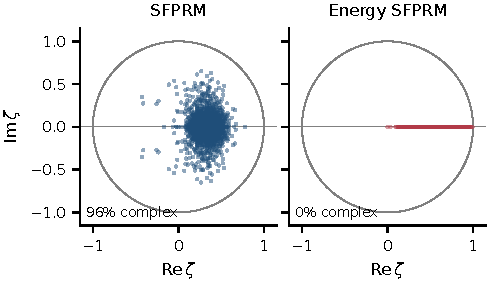
\includegraphics[width=\columnwidth]{figures/spectrum_4x4v2.pdf}\\[2pt]
  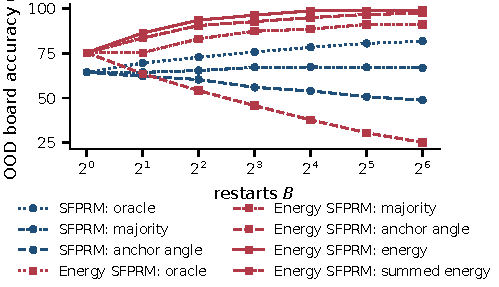
\includegraphics[width=\columnwidth]{figures/restarts_4x4v2.pdf}
  \caption{Codebook variant against SFPRM on $4\times4$ Sudoku. Top: eigenvalues of the tangent
  Jacobian at polished halted OOD states (three puzzles pooled); SFPRM at $\eta=1$, the energy model
  for the damped map at $\eta=1/\lambda_{\max}(\operatorname{Hess}E)$, half its window. Bottom: OOD
  board accuracy against the number of restarts $B$ under the selection rules of
  \cref{prop:voting}; lowest-energy selection coincides with the oracle.}
  \label{fig:codebook}
\end{figure}

The memory term has a probabilistic reading that suggests three further changes. With memories of
fixed norm $\norm{\xi_\mu}=r$, $e^{\beta\ip{\xi_\mu}{z}}$ is, up to normalization, a von
Mises--Fisher density on $\Sph^{d-1}$ with mean direction $\xi_\mu/r$ and concentration $\beta r$
\citep{mardia2000}, so $E_M(z_t)=-\tfrac1\beta\log p(z_t)+\mathrm{const}$ for an equal-weight
vMF mixture centred on the memories, and the memory step is Riemannian gradient ascent on a learned
mixture density. Each term of \eqref{eq:energy} then has a role in a continuous relaxation of a
discrete constraint problem: the injection is the evidence, the attention energy holds the pairwise
constraints, and the memory is a unary potential whose minima are the codebook points. At large
$\beta$ the memory energy of a token approaches $-\max_\mu\ip{\xi_\mu}{z_t}$, a pinning potential
toward the nearest prototype, the learned analogue of the sub-harmonic injection locking that
oscillator Ising machines use to force continuous phases onto discrete values \citep{wang2019oim}.
This motivates the following \emph{codebook variant} of \cref{def:esfprm}.
\emph{Answer codebook and tied readout.} An extra memory term
$E_{\mathrm{ans}}(z)=-\tfrac{\kappa_{\mathrm{ans}}}{\beta_{\mathrm{ans}}}\sum_t\log\sum_{k=1}^{n}e^{\beta_{\mathrm{ans}}\ip{\xi^{\mathrm{ans}}_k}{z_t}}$
on the visible tokens has one unit-norm prototype per output symbol; the readout is
$\mathrm{logits}_t=s\,\Xi^{\mathrm{ans}}z_t$, so the prediction is the prototype the token sits in,
the cross-entropy trains the prototypes directly, and the digit embedding of the input shares the
same prototypes. \emph{Commitment.} $c_t=\max_k\operatorname{softmax}(\beta_{\mathrm{ans}}\Xi^{\mathrm{ans}}z_t)_k$
is a label-free certificate; a token is committed when $c_t>1-\epsilon$, and ``residual below
$\tau$ and every token committed'' is a stronger halting test than the residual alone.
\emph{Annealing.} $\beta$ controls the landscape \citep{ramsauer2021hopfield}: small $\beta$ gives a
single smooth minimum near the mean of the memories, large $\beta$ one minimum per memory. A
schedule $\beta_i=\beta\,\rho^{-(1-\min(i/K,1))}$ over iterations lets coupling and injection act
first and commits tokens late; like an annealed frequency (\cref{sec:oscillatory}) it cannot be
folded into the weight-tied block, and \cref{thm:lyapunov} applies once the schedule has ended.
\emph{Ranking loss.} To make the premise of \cref{prop:voting} hold, training adds, over $R$
restarts of the same puzzle, the hinge $\max(0,E(w^\star_{\mathrm{correct}})-E(w^\star_{\mathrm{wrong}})+m)$
whenever both kinds of halted state occur, so that the energy learns to rank solutions.
\Cref{tab:results} repeats the pilot protocol for the codebook variant and \cref{fig:codebook}
shows its $4\times4$ spectrum and restart curves; \cref{app:pilot} has the training and halting
curves. Five findings.
\emph{The codebook changes the picture.} Without the ranking loss the variant solves $98.0\%$ of
ID and $74.4\%$ of OOD boards on $4\times4$ with one restart, against $97.8\%$ and $65.6\%$ for SFPRM
and $82.4\%$ and $17.2\%$ for the first energy model, and it trains in fewer steps than the first
energy model.
\emph{Energy selection now works.} Selecting the lowest-energy halted state among $B$ restarts
matches the oracle at every $B$: OOD accuracy rises from $75.4\%$ at $B=1$ to $99.0\%$ at $B=64$,
whereas majority voting reaches $91.2\%$ and anchor-angle selection falls to $25.2\%$. SFPRM's best
rule at $B=64$ reaches $67.0\%$ and its oracle $81.8\%$ (\cref{fig:codebook}). The premise of
\cref{prop:voting} holds for the learned energy: whenever a restart finds the solution, it is the
lowest minimum.
\emph{The schedule is necessary, the ranking loss is not.} With $\beta$ fixed at its final value from
the first iteration the variant never leaves the plateau (no board solved, no puzzle halted, in
$2{,}000$ steps): tokens commit to prototypes before attention can propagate the constraints. The ranking loss does not improve
selection, which already matches the oracle without it, and it costs single-restart accuracy
($94.6\%$ / $62.8\%$ with it, although it places the correct state lower in energy for $88\%$ of
training pairs); energy selection behaves well because the readout and the energy share the
prototypes, not because ranking is trained explicitly.
\emph{Commitment certifies.} At the halted state, $75.6\%$ of committed OOD boards are correct and
none of the uncommitted ones. Requiring commitment in the halting test does not help, however: it
lowers board accuracy by $0.4$--$3.0$ points, since almost every state that passes the residual test
is already committed.
\emph{Spectrum and halting.} All eigenvalues at halted states are real, as \cref{prop:real-spectrum}
requires, and Armijo backtracking halts $98\%$ of the OOD puzzles, against $24\%$ for the patience
rule. The learned Hessian remains stiff ($\lambda_{\max}\approx13$), so halting takes a median of
$43$ OOD iterations against $19$ for SFPRM; the $\beta$ schedule does not remove the stiffness.
Replacing only SFPRM's MLP by a tied memory, without any energy, costs a third of the parameters and
some accuracy ($95.8\%$ / $55.0\%$ on $4\times4$, $99.2\%$ / $69.8\%$ on $6\times6$) and leaves
$94\%$ of the eigenvalues complex: the benefits above come from the energy, not from the memory
layer alone.
\emph{$6\times6$.} The first energy model solved no $6\times6$ board; the codebook variant (trained
with the ranking loss) reaches $61.2\%$ ID and $11.0\%$ OOD with one restart, below SFPRM's
$99.8\%$ and $89.2\%$, and its training accuracy was still rising when the $4{,}000$-step budget
ended. Energy selection again tracks the oracle: over $64$ restarts it reaches $100\%$ ID and
$88.2\%$ OOD (oracle $100\%$ and $89.8\%$), against $59.4\%$ for majority voting and $0.4\%$ for
the anchor angle OOD, and just below SFPRM's best rule at $B{=}64$ ($92.8\%$). The spectrum is again
real, halting is again slow (median $103$ OOD iterations), and $98\%$ of committed ID boards are
correct against $52\%$ of uncommitted ones.

